\chapter{Case Study on Resource-centric Organizational Modeling}
\label{chap:casestudy}
In this chapter, we provide architecture of the functioning system as a first section. This section provides, implementation details along with the reason for making certain decisions regarding the implementation. The second section explain how motivating scenario has been realized using the proposed modeling approach. Successful modeling of the motivating scenario using the developed editor serves as a proof for usability of the web editor. Hence the final section validates the system by validating it with the proposed approach. This section also has some requirement evaluation with the state of the art approaches.

%%%%%%%%%%%%%%%%%%%%%%%%%%%%%%%%%%%%%%%%%%%%%%%%%%%%%%%%%%%%%%%%%%%%%%%%%
\section{Architecture of the Functioning System}
\label{sec:architectureofthefunctioningsystem}
%%%%%%%%%%%%%%%%%%%%%%%%%%%%%%%%%%%%%%%%%%%%%%%%%%%%%%%%%%%%%%%%%%%%%%%%%
As discussed in the Chapter \ref{chap:approach}, informal process targets for accomplishment of an intention. Thus in the Figure \ref{fig:architectureofthecasestudy}, we associate intentions with both process definitions and strategy definitions as intention definitions are used by both process definitions and strategy definitions. Intentions are associated to resources either through strategies or through informal processes. Intentions can be refined by defining sub-intentions, which can be defined recursively as independent informal process. For example, in our motivating scenario the main intention increase revenue and number of unit sales can be refined into sub-intention of improve customer help desk portal. This sub-intention can be associated with process models. This \textit{intention-based} approach enables describing process declaratively,  i.e., without describing \textit{how} the intention is achieved, and providing information about \textit{what} has to be achieved. This avoids the need for predefined business logic in the representations of informal process \cite{Sungur2014a}. 

\begin{figure}
	\centering
	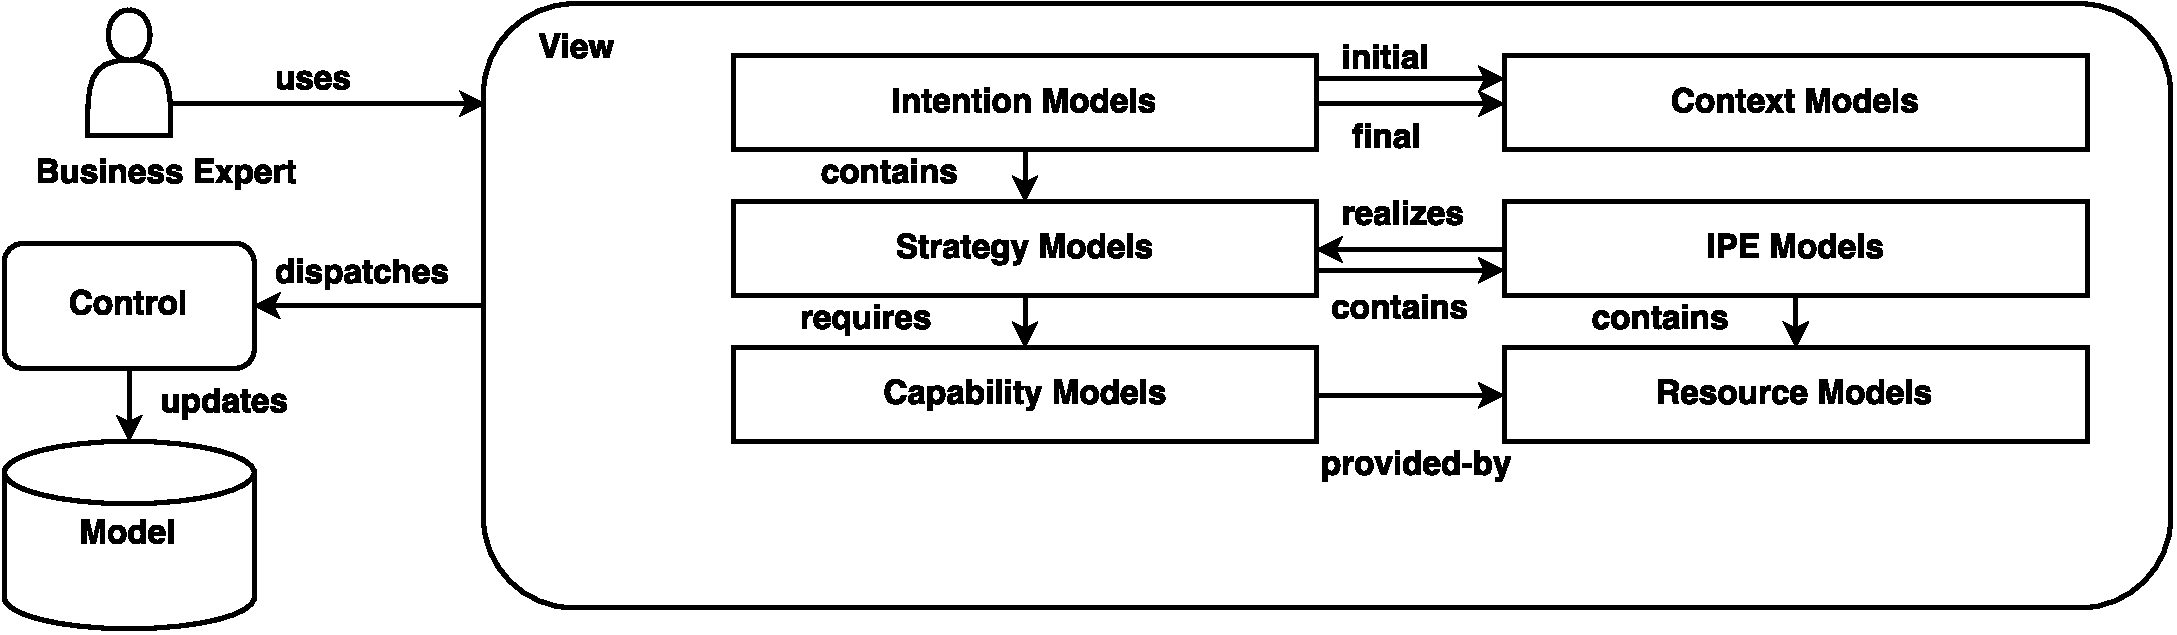
\includegraphics [width= \textwidth]{architectureofthecasestudy.pdf}
	\caption{Architecture of the Functioning System}
	\label{fig:architectureofthecasestudy}
	\end{figure}

Also from the Figure \ref{fig:architectureofthecasestudy}, it is clear that we followed the MVC architecture to design the user interface. Business experts can use the editor to view/update the descriptive entity details. Whenever a change in the model data is detected respective handler function is \textit{dispatched} and the corresponding handler function can only \textit{update} the model. Since we associate every entity type with another entity type, model data of an entity type is required by another entity type which are resolved using the unique reference identifier. For example, intention model's unique reference identifier of intention \textit{improve help customer help portal} is required by the strategy \textit{through application development}. This is because for strategy (through application development), intention (improve help customer help portal) is the target intention. 

%%%%%%%%%%%%%%%%%%%%%%%%%%%%%%%%%%%%%%%%%%%%%%%%%%%%%%%%%%%%%%%%%%%%%%%%%
\section{Technologies and Frameworks}
\label{subsec:specifications}
%%%%%%%%%%%%%%%%%%%%%%%%%%%%%%%%%%%%%%%%%%%%%%%%%%%%%%%%%%%%%%%%%%%%%%%%%
In order to realize the web-based editor of resource-centric organizational modeling, a formal inquiry was done to choose suitable technologies and frameworks required. The below specifications were finalized and \textit{client-side scripting}\footnote{https://en.wikipedia.org/wiki/Client-side\_scripting} was chosen, due to the fact that our developed editor is web-based. 

\begin{enumerate}   
	\item \textit{ClojureScript}\footnote{http://clojure.org/about/clojurescript} as the programming language
	\item \textit{Model-view-controller (MVC)}\footnote{https://en.wikipedia.org/wiki/Model-view-controller}  as the architecture pattern
	\item \textit{Re-frame}\footnote{https://github.com/Day8/re-frame} as the pattern for writing SPAs \footnote{https://en.wikipedia.org/wiki/Single-page\_application} in ClojureScript, using Reagent	
\end{enumerate}

Other than the above listed frameworks and technologies, frameworks like \textit{react-bootstrap}\footnote{https://react-bootstrap.github.io/}, jquery\footnote{https://jquery.com/} were also used to provide more optimal view of the editor. Along with this we have also used libraries like bidi\footnote{https://github.com/juxt/bidi} and pushy\footnote{https://github.com/kibu-australia/pushy}, to handle page navigation fom current location to the desired location in the URL\footnote{URL- Uniform Resource Locator} of the browser. \textit{Clojure} is a dynamic, general-purpose programming language, combining the approachability and interactive development of a scripting language with an efficient and robust infrastructure for multithreaded programming. \textit{ClojureScript} is a compiler for Clojure that targets JavaScript which has been designed to emit JavaScript code. In our implementation, we have used both Clojure and Clojurescript. We also used \textit{Reagent}\footnote{http://reagent-project.github.io/} which provides a minimalistic interface between ClojureScript and React\footnote{https://facebook.github.io/react/}. A \textit{Re-frame}\footnote{https://github.com/Day8/re-frame} is a pattern for writing applications in ClojureScript, using Reagent.

%%%%%%%%%%%%%%%%%%%%%%%%%%%%%%%%%%%%%%%%%%%%%%%%%%%%%%%%%%%%%%%%%%%%%%%%%
\subsection{MVC Architecture}
\label{subsec:mvcarch}
%%%%%%%%%%%%%%%%%%%%%%%%%%%%%%%%%%%%%%%%%%%%%%%%%%%%%%%%%%%%%%%%%%%%%%%%%
The architecture of the developed user interface is based on the \textit{Model-View-Control (MVC)} design pattern. The MVC paradigm allows to separate business logic from the code that controls presentation and event handling \cite{Oracle2016}. Each entity view in the web page is made up of combination of at least one Model and View, and one or more Controls. 

\textit{Model} artifact stores the required data structure for web-editor. In the developed model artifact, the four main types of data structure such as intentions, strategies, capabilities and informal process instances are stored. 

\textit{View} artifact contains HTML\footnote{https://en.wikipedia.org/wiki/HTML} elements and HTML constructs that describe the way of displaying the data from Model to the user. Most of the common functionalities that render user interface components are re-used. 

\textit{Control} artifact contains the handler functions which can only change the model. Even the initial values of the model are put inside the control. This artifact has functions that updates default database, which then causes a re-render of view that makes the user to see a new view.

Apart from the above artifacts, there is another important artifact that registers subscription functions i.e., query layer of the data. As view components never source data directly from default model, we use \textit{subscription} functions. Subscription functions returns values that change over time i.e based on a user events.

%%%%%%%%%%%%%%%%%%%%%%%%%%%%%%%%%%%%%%%%%%%%%%%%%%%%%%%%%%%%%%%%%%%%%%%%%
\subsubsection{Example: Component using MVC Pattern }
%%%%%%%%%%%%%%%%%%%%%%%%%%%%%%%%%%%%%%%%%%%%%%%%%%%%%%%%%%%%%%%%%%%%%%%%%
The Figure \ref{fig:mvc_arch} below shows the simplifed version of how the components interact with each other using the Model-View-Control (MVC) pattern, for the functionality of adding new entity data. This functionality is same for all the types such as intentions, strategies, capabilities and informal processes and below is the detailed explanation of each interaction.

\begin{figure}
	\centering
	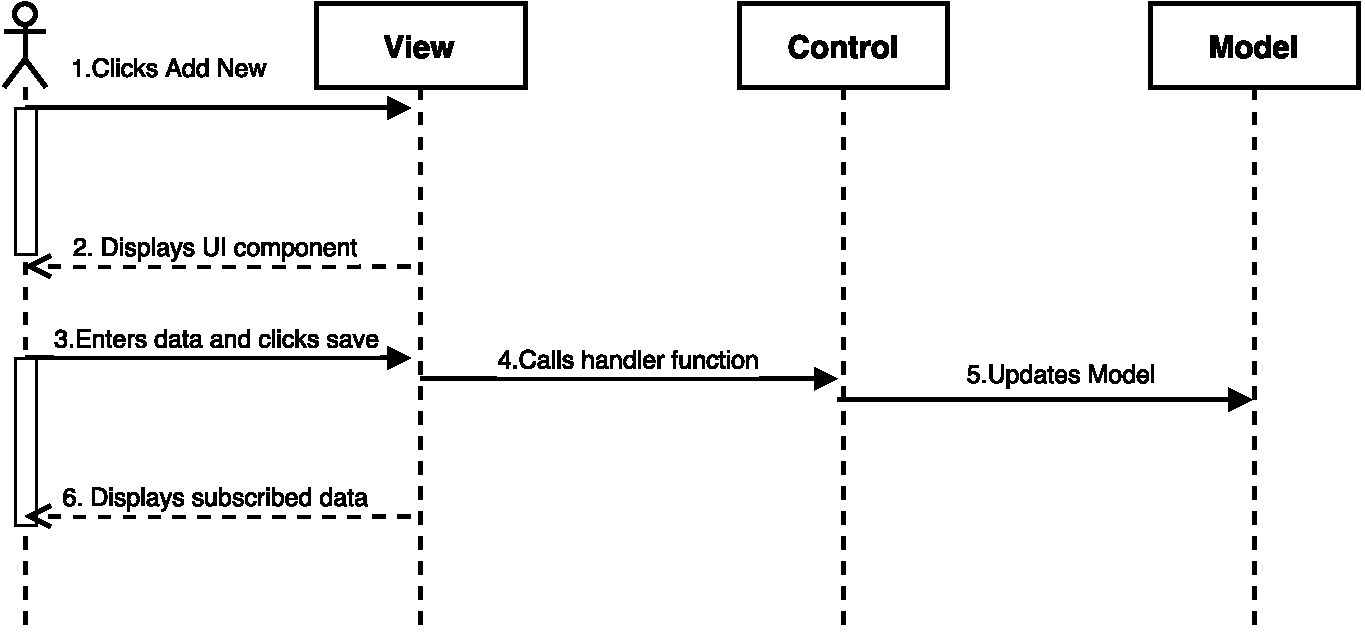
\includegraphics [width= \textwidth]{mvc_pattern.pdf}
	\caption{MVC Pattern of adding new entity}
	\label{fig:mvc_pattern}
\end{figure}

\begin{enumerate}
	\item User clicks the tab \textit{Add New} button in the developed editor.
	\item In response to the user click, the view displays the respective user interface component for entering the new entity data details.
	\item User enters the required basic details for adding new entity data and clicks save button.
	\item The view dispatches the data to control, as control can only modify the model.
	\item Control inserts/updates data into the model.
	\item View displays the updated model as it has been subscribed to the model.
\end{enumerate}


%%%%%%%%%%%%%%%%%%%%%%%%%%%%%%%%%%%%%%%%%%%%%%%%%%%%%%%%%%%%%%%%%%%%%%%%%
\subsection{Application Flow}
\label{subsec:applicationflow}
%%%%%%%%%%%%%%%%%%%%%%%%%%%%%%%%%%%%%%%%%%%%%%%%%%%%%%%%%%%%%%%%%%%%%%%%%
In this sub section we provide an overview about how page navigation from current location to the desired location happen in URL\footnote{URL- Uniform Resource Locator} of the browser. The external libraries used for route navigation, parses URLs into data structures and also generates URLs from data structure defined as required routes. We call a function to dispatch route, with the matched route. Then we also have function that parses the URL, to turn a URL into a data structure representing it. From the Figure \ref{fig:UIArchitecture}, it is clear that route navigation for each entity items happens based on their entity type and its own unique reference identifier.

\begin{figure}
	\centering
	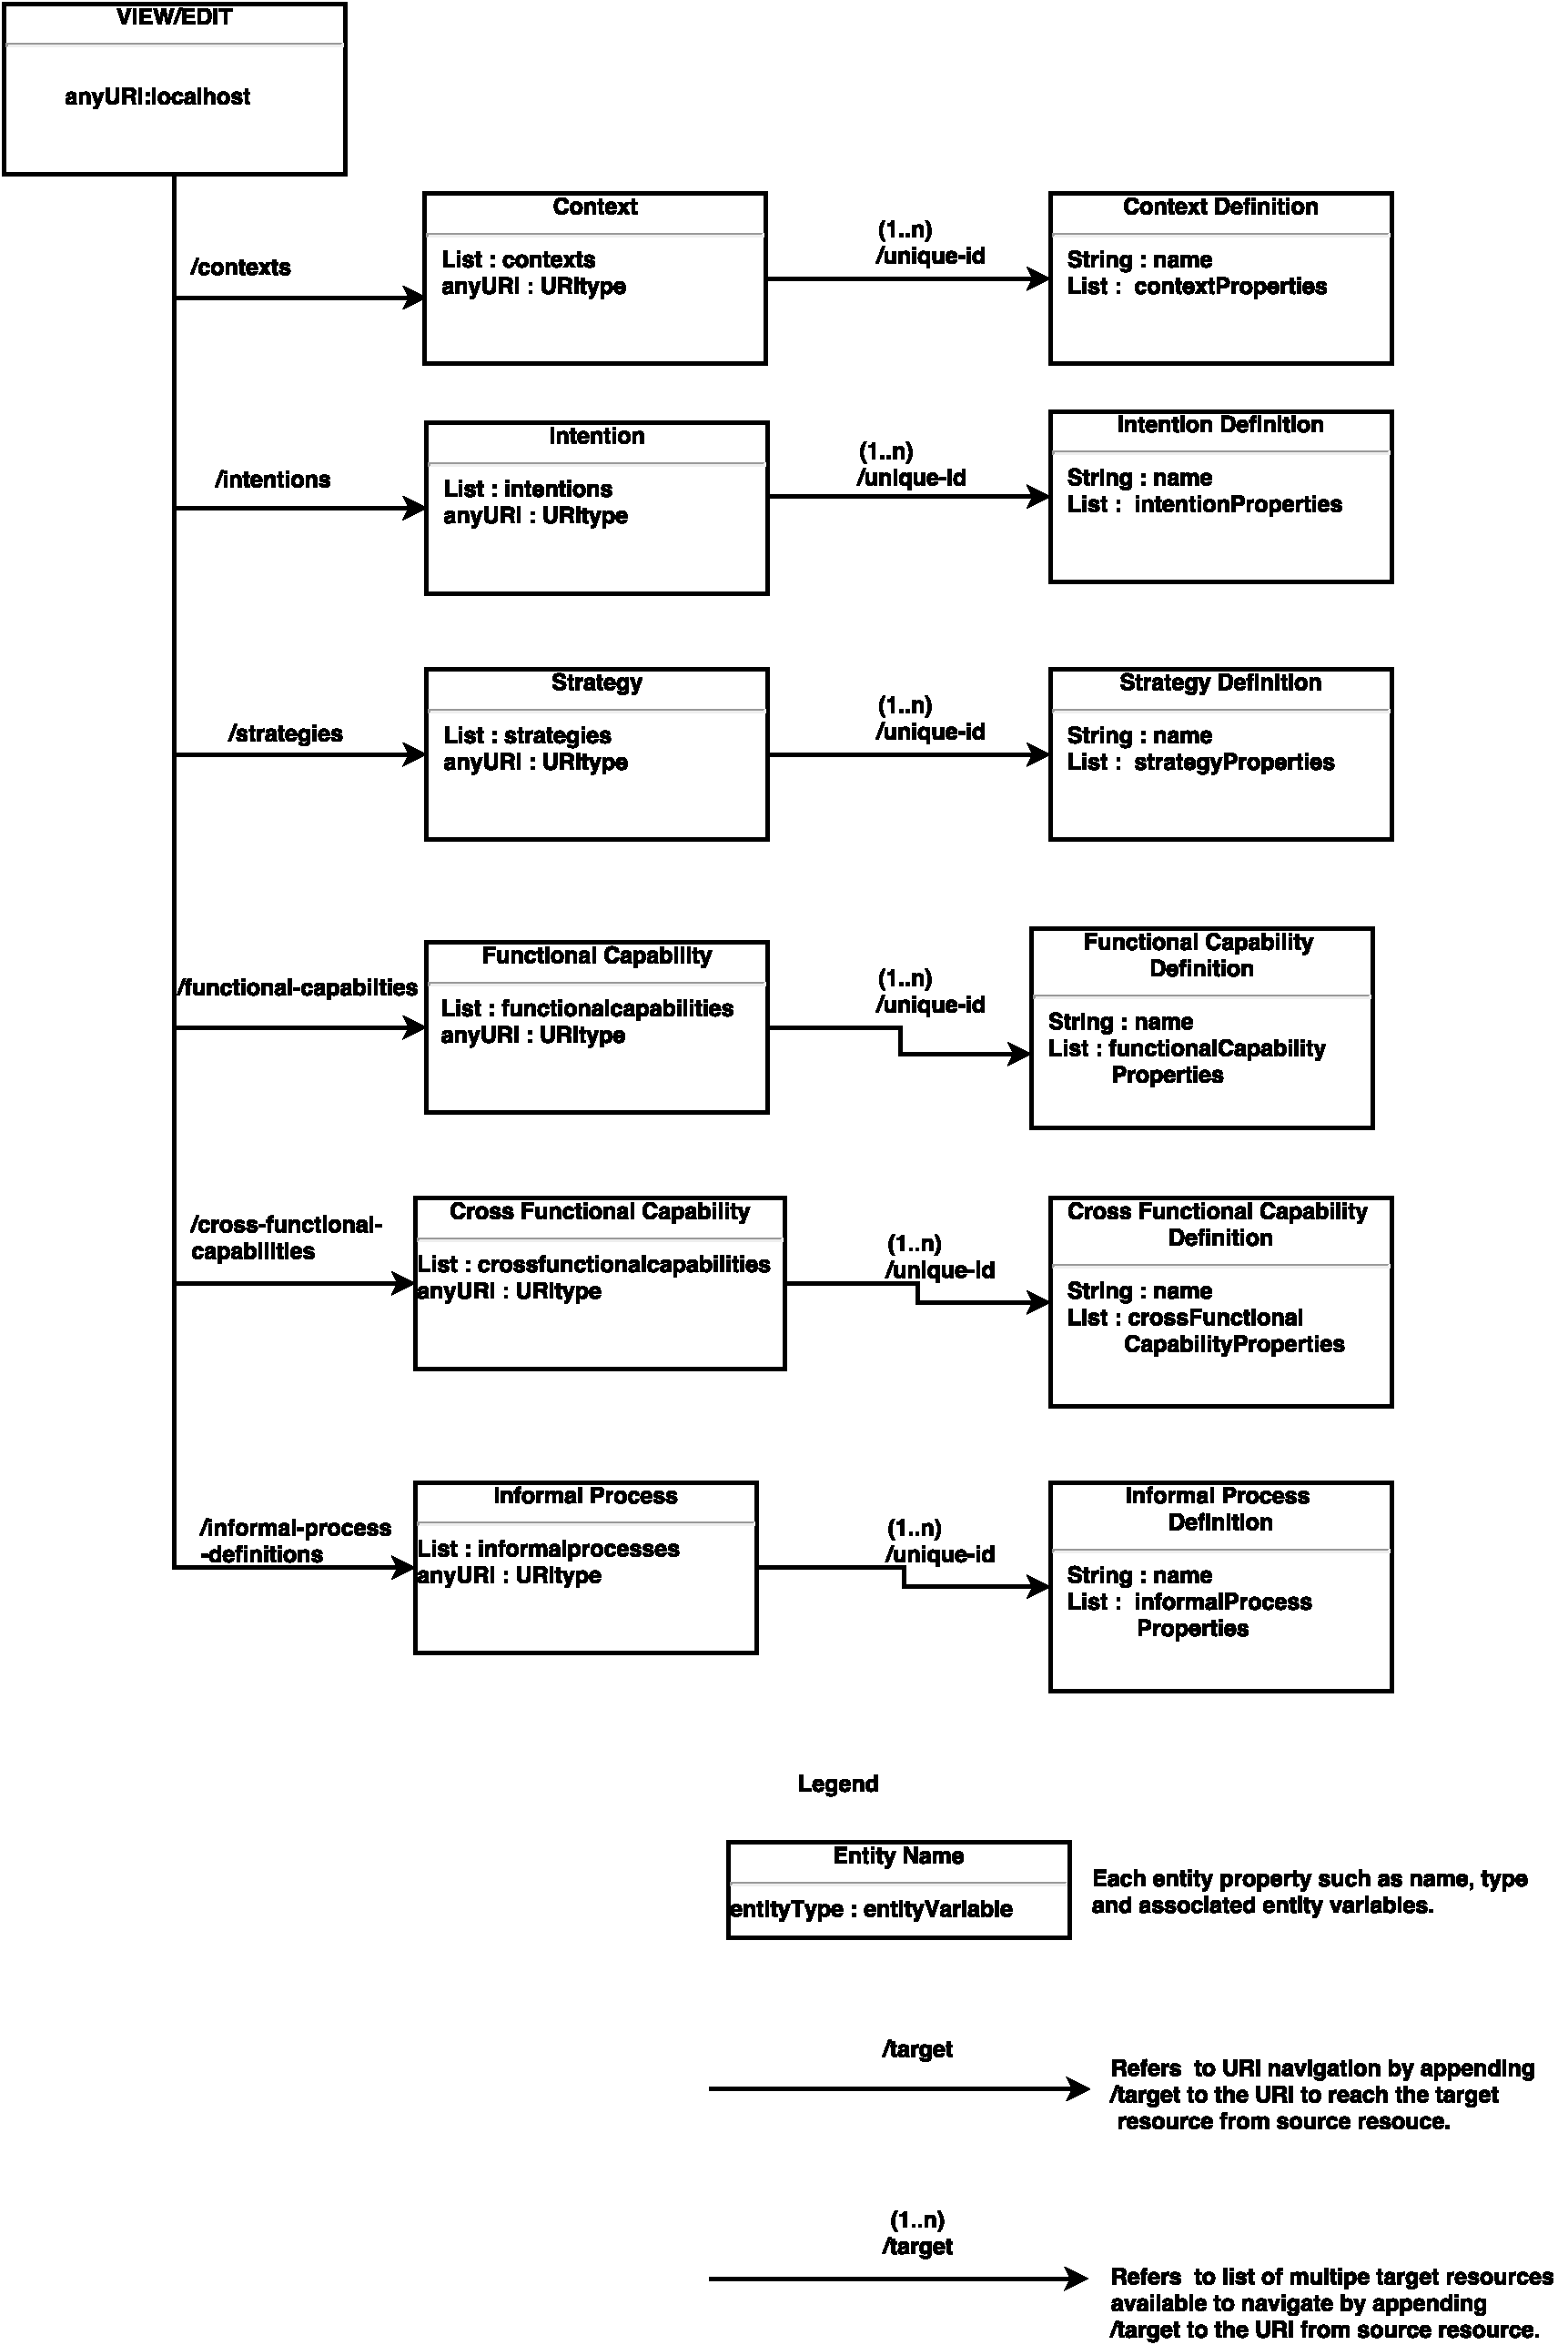
\includegraphics [width= \textwidth]{UIArchitecture.pdf}
	\caption{User interface URL navigation of the functioning system}
	\label{fig:UIArchitecture}
\end{figure} 

Each entity item has basic properties such as \textit{name} and \textit{target namespace}. The entities are identified using their unique id which is generated using the combination of name and target namespace. Other entities that are associated with a particular entity are resolved through this unique identifier. For example, in our motivating scenario consider the intention \textit{improve the customer help desk portal} when creating model for this intention, business expert provide name and namespace for this intention and add it to the database. A unique identifier is generated for the intention model using the combination of name and namespace by the system. The strategy (in our scenario \textit{through application  development}) that is associated with this intention, just contains only this unique identifer for the reference. 

%%%%%%%%%%%%%%%%%%%%%%%%%%%%%%%%%%%%%%%%%%%%%%%%%%%%%%%%%%%%%%%%%%%%%%%%%
\section{A Concrete View of Entity Types}
\label{sec:concreteviewofentitytypes}
%%%%%%%%%%%%%%%%%%%%%%%%%%%%%%%%%%%%%%%%%%%%%%%%%%%%%%%%%%%%%%%%%%%%%%%%%
It is important to discuss the concrete concepts of informal process from an organizational aspects, because organizational aspects have a direct effect on the outcome of the informal process \cite{Sungur2014}. This section discusses about how resource-centric organizational modeling is realized as a web-based editor from an organizational aspect by taking the motivating scenario discussed in Chapter \ref {chap:motivatingScenario}. Though developing schema definitions are not part of the thesis implementation, it has been provided because the editor has a view that is capable of adding, viewing, deleting and updating model data aligned with the schema definition. A typical XML Schema Definition of entity type has been provided in the listing \ref{lst:xsdlist}.

\begin{Listing}
	\begin{lstlisting}
	<xs:complexType name="tEntityType" abstract="true">
	<xs:complexContent>
	<xs:extension base="tExtensibleElements">
	<xs:sequence>
	<xs:element name="Tags" type="tTags" minOccurs="0"/>
	<xs:element name="DerivedFrom" minOccurs="0">
	<xs:complexType>
	<xs:attribute name="typeRef" type="xs:QName" use="required"/>
	</xs:complexType>
	</xs:element>
	<xs:element name="PropertiesDefinition" minOccurs="0">
	<xs:complexType>
	<xs:attribute name="element" type="xs:QName"/>
	<xs:attribute name="type" type="xs:QName"/>
	</xs:complexType>
	</xs:element>
	</xs:sequence>
	<xs:attribute name="name" type="xs:NCName" use="required"/>
	<xs:attribute name="abstract" type="tBoolean" default="no"/>
	<xs:attribute name="final" type="tBoolean" default="no"/>
	<xs:attribute name="targetNamespace" type="xs:anyURI" use="optional"/>
	</xs:extension>
	</xs:complexContent>
	</xs:complexType>>
	\end{lstlisting}
	\caption{XML Schema Definition of Entity Type}
	\label{lst:xsdlist}
\end{Listing}

%%%%%%%%%%%%%%%%%%%%%%%%%%%%%%%%%%%%%%%%%%%%%%%%%%%%%%%%%%%%%%%%%%%%%%%%%
\section{Realization of Motivating Scenario}
\label{sec:realization}
%%%%%%%%%%%%%%%%%%%%%%%%%%%%%%%%%%%%%%%%%%%%%%%%%%%%%%%%%%%%%%%%%%%%%%%%%
The realization of motivating scenario is explained by integrating the concepts discussed in Chapter \ref{chap:motivatingScenario} and the informal process modeling approach discussed in Chapter \ref{chap:fundamentals}. From the Figure \ref{fig:realizationofmotivatingscenario}, it is clear that to realize the motivating scenario using the proposed approach it is important to model them step by step as mentioned in the informal process modeling approach. The developed editor also supports dynamic changes in the models whenever there is a need to add new models. As each models are designed in individual modeling step, details of individual modeling steps are provided in the following sub sections. 

\begin{figure}
	\centering
	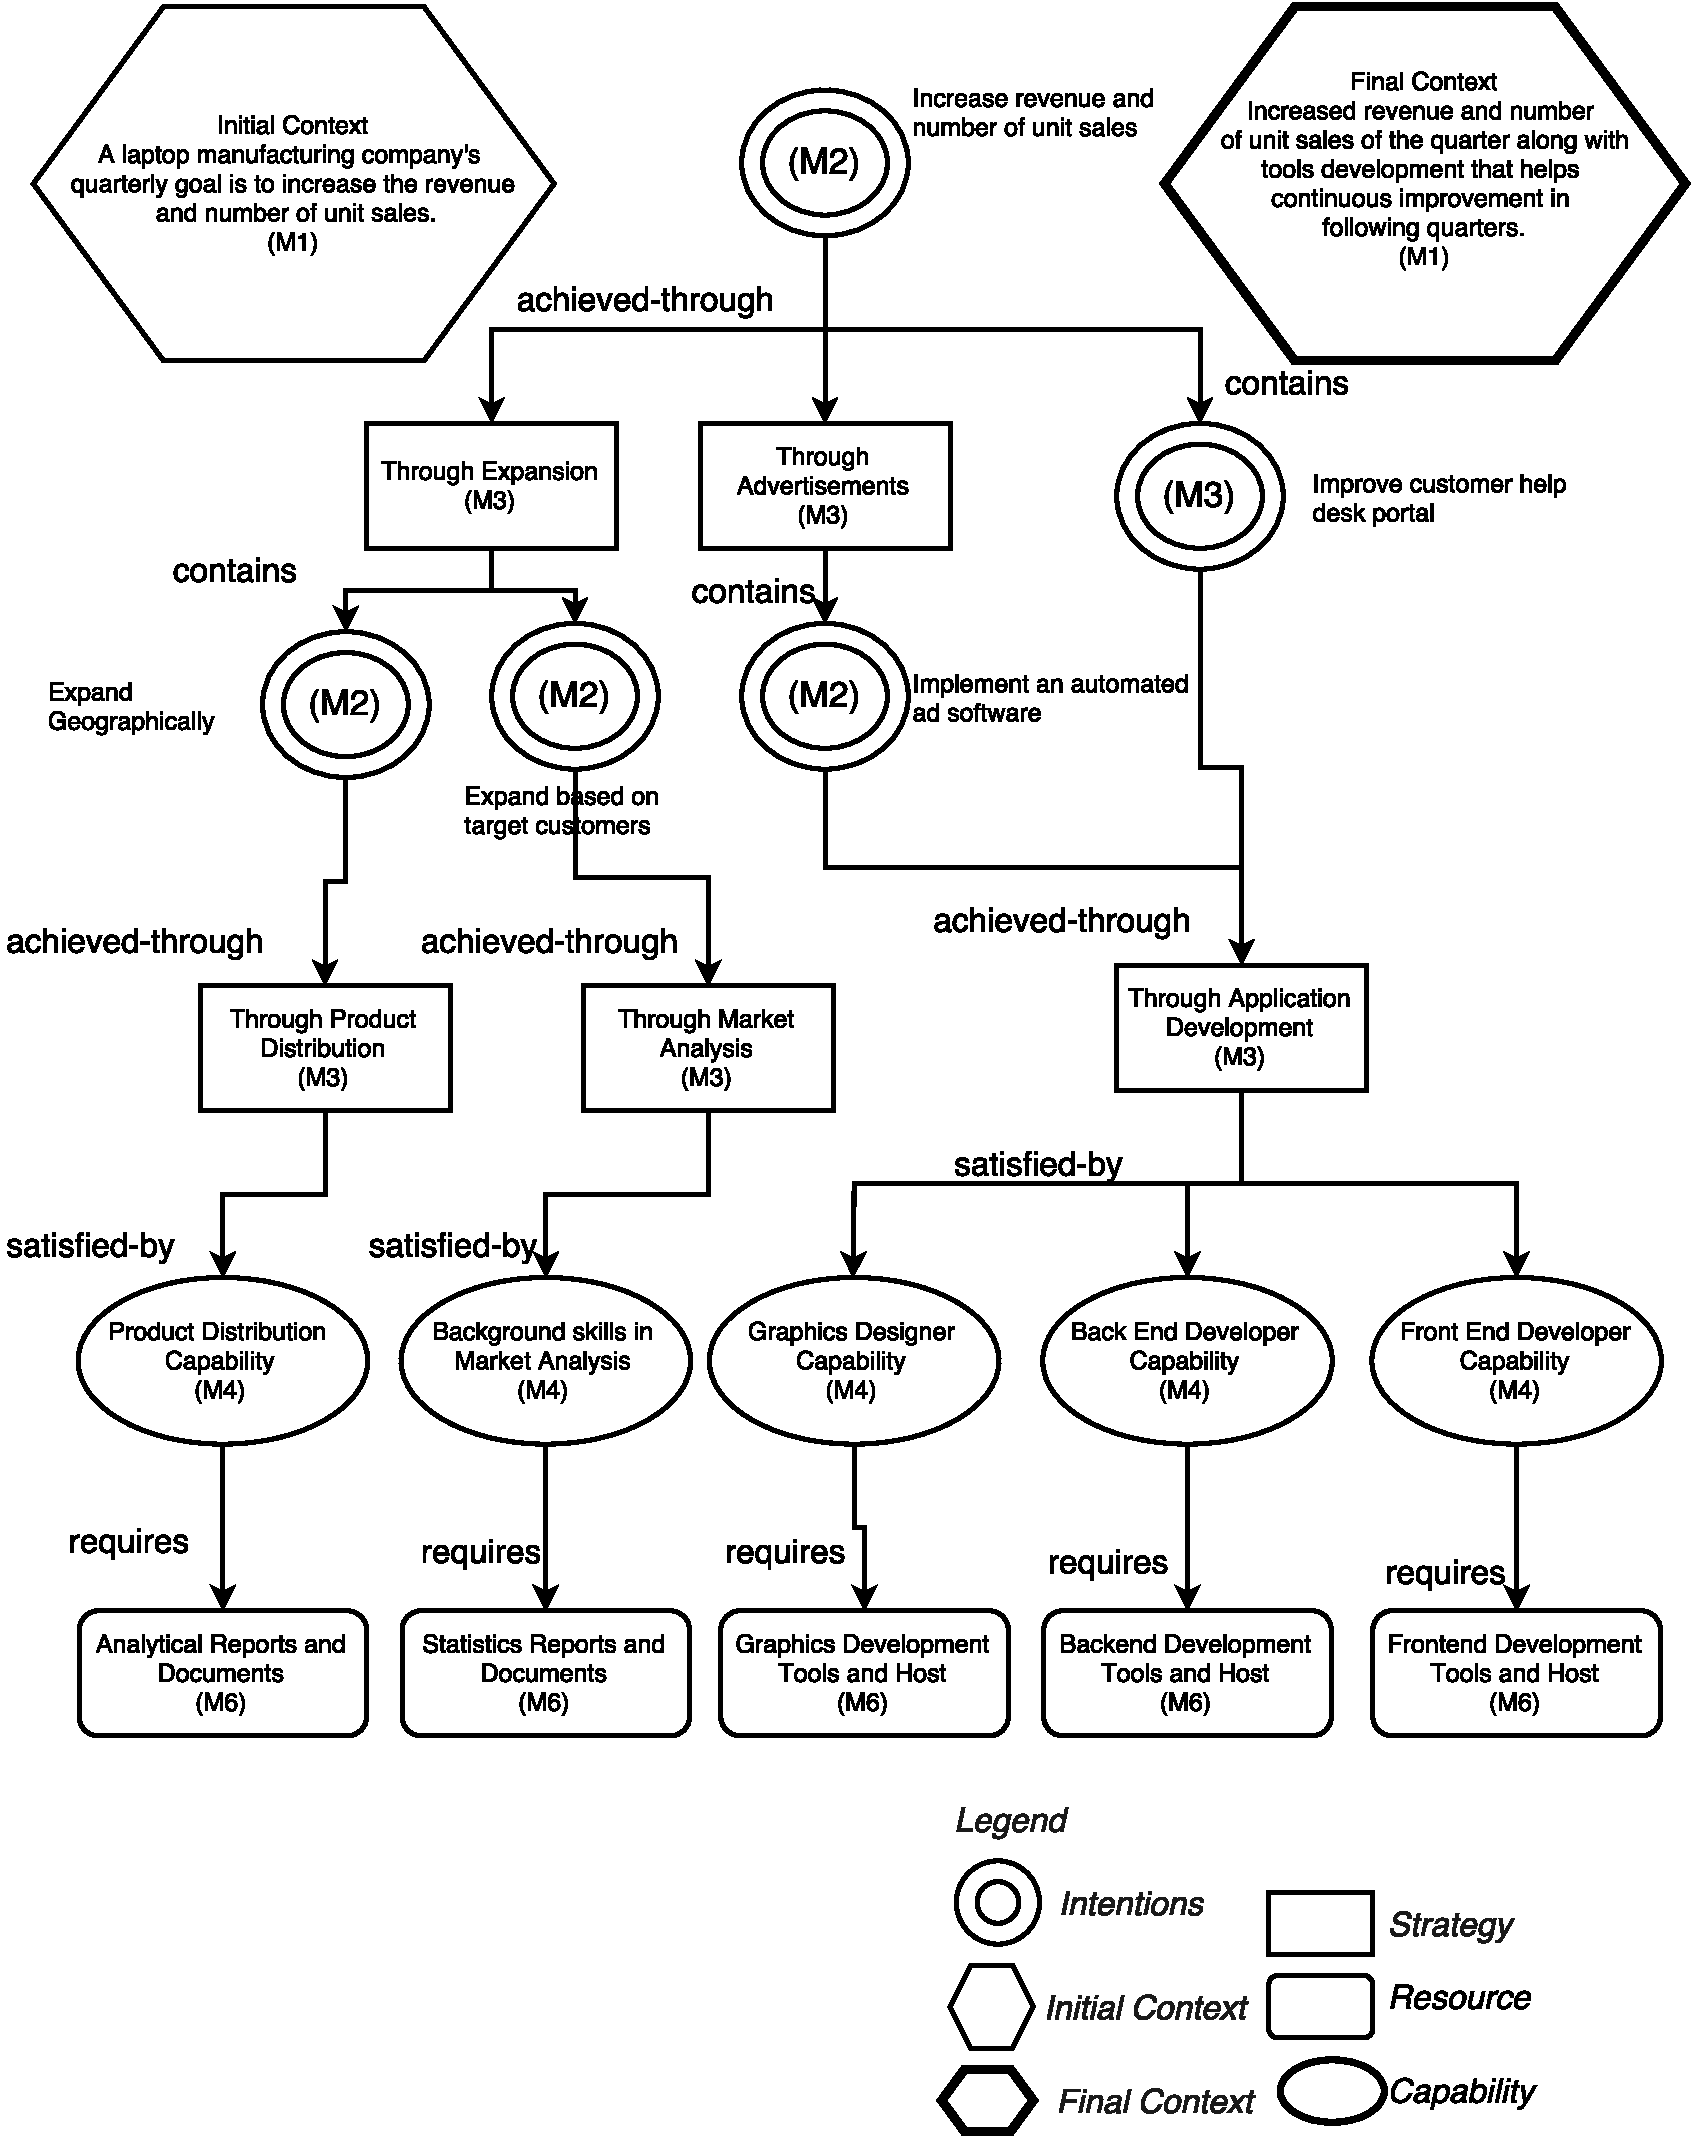
\includegraphics[width=\textwidth,angle=0]{PhasesofMotivatingScenario.pdf}
	\caption{Realization of Motivating Scenario}
	\label{fig:realizationofmotivatingscenario}
\end{figure}

%%%%%%%%%%%%%%%%%%%%%%%%%%%%%%%%%%%%%%%%%%%%%%%%%%%%%%%%%%%%%%%%%%%%%%%%%
\subsection{Realization of Context Definitions}
%%%%%%%%%%%%%%%%%%%%%%%%%%%%%%%%%%%%%%%%%%%%%%%%%%%%%%%%%%%%%%%%%%%%%%%%%
In the informal process modeling approach, the first modeling step is to model the context definitions(M1). Each informal process starts from an initial context, i.e., IPE Context and aims to achieve an intention, i.e., an IPE Intention \cite{Sungur2014a}. After reaching an intention, there is resulting IPE Context. In the motivating scenario, the user can add new contexts by providing basic properties such as name of the context and target namespace of the context as they serve as unique reference identifier for these contexts. After successfully adding the basic properties, user can provide entity specific properties such as contained contexts inside the main context, entity definition details about the contexts and participant list such as which user has what type of privileges. The required context definitions are modeled first because these definition are required for modeling intention definitions and process definitions.  

%%%%%%%%%%%%%%%%%%%%%%%%%%%%%%%%%%%%%%%%%%%%%%%%%%%%%%%%%%%%%%%%%%%%%%%%%
\subsection{Realization of Intention Definitions}
%%%%%%%%%%%%%%%%%%%%%%%%%%%%%%%%%%%%%%%%%%%%%%%%%%%%%%%%%%%%%%%%%%%%%%%%%
After modeling context definitions(M1), the second step of the modeling is to model the intentions(M2). For example, in our motivating scenario we have main intention of "increase revenue and number of unit sales" and other sub-intentions that are emerged out of main intentions and strategies of the main intention. The user can provide descriptive information about particular intention as intention definition. Similar to context modeling, the user has to provide basic properties such as name and target namespace required for unique identification of this entity. After providing basic properties, the user has to provide entity specific details of the intention such as due date and time for intention completion, priority of the intention, cost of the intention, sub intentions that are contained under this particular intention and how the sub-intentions are related to this intention. The strategies to achieve this intention and contexts of the intention are also provided as entity specific properties. The participant list with respective privileges for each participant are also provided. 

%%%%%%%%%%%%%%%%%%%%%%%%%%%%%%%%%%%%%%%%%%%%%%%%%%%%%%%%%%%%%%%%%%%%%%%%%
\subsection{Realization of Strategy Definitions}
%%%%%%%%%%%%%%%%%%%%%%%%%%%%%%%%%%%%%%%%%%%%%%%%%%%%%%%%%%%%%%%%%%%%%%%%%
After modeling context definitions(M1) and intention definitions(M2) user can proceed to model the strategies through which an intention can be achieved which is third step of the modeling process. For example, in our motivating scenario user can model the strategies such as \textit{through expansion},\textit{through advertisements} and other required strategies as third step of the modeling process. Similar to earlier modeling steps, during the modeling of strategy also user required to provide basic properties such as name and target namespace. After providing the basic properties, entity specific properties such as target intention of the strategy, intention, capability and process definitions associated with strategy are also provided. Since strategy is also an interactive acquirable entity similar to intention, participant list details are also provided during modeling of strategies

%%%%%%%%%%%%%%%%%%%%%%%%%%%%%%%%%%%%%%%%%%%%%%%%%%%%%%%%%%%%%%%%%%%%%%%%%
\subsection{Realization of Capabilitiy Definitions}
%%%%%%%%%%%%%%%%%%%%%%%%%%%%%%%%%%%%%%%%%%%%%%%%%%%%%%%%%%%%%%%%%%%%%%%%%
There are two types of capabilities. Functional capabilities and cross-functional capabilities. Functional capabilities are the capabilites that associated with other entity types. Cross-functional capabilities contains multiple functional capabilities. Similar to earlier entity types basic properties such as name and target namespace are added to get the unique reference identifier and entity specific properties for both capabilities are added. Since cross functional capability contains functional capabilities, it holds the identifiers of the functional capabilities contained in it. Functional capability definitions also has participant list details similar to intention definitions and strategy definitions. 

%%%%%%%%%%%%%%%%%%%%%%%%%%%%%%%%%%%%%%%%%%%%%%%%%%%%%%%%%%%%%%%%%%%%%%%%%
\subsection{Realization of Process Definitions}
%%%%%%%%%%%%%%%%%%%%%%%%%%%%%%%%%%%%%%%%%%%%%%%%%%%%%%%%%%%%%%%%%%%%%%%%%
By modeling the business processes based on the resources that work towards certain intentions, informal processes are modeled without predefining their business logic \cite{Sungur2014a}. Also as mentioned earlier each informal process starts from an initial context and aims to achieve an intention that results in a final context. Thus we require context definitions and intention definitions before modeling process definitions. Similar to earlier modeling of entity types, process modeling also require basic properties such as name and namespace  and entity specific properties such as associated intentions, contexts and resources. Process definition also has participant list similar to other entity types. 

%%%%%%%%%%%%%%%%%%%%%%%%%%%%%%%%%%%%%%%%%%%%%%%%%%%%%%%%%%%%%%%%%%%%%%%%%
\subsection{Realization of Resource Definitions}
%%%%%%%%%%%%%%%%%%%%%%%%%%%%%%%%%%%%%%%%%%%%%%%%%%%%%%%%%%%%%%%%%%%%%%%%%
As discussed earlier each resource can be related to another resource which are defined using predefined or custom \textit{relationships} \cite{Sungur2014a}. These resources are managed through \textit{Resource Organizers}, this is because resource organizers are used to bring together the relevant interrelated resources that work towards to achieve the corresponding intentions. TOSCA \cite{Binz2014} can be used to model all nodes and relationship among them. In this work, consider resources as nodes to make use of the TOSCA's service. The schema definition of considering each resource as node is provided in the listing \ref{lst:xsdnodetype}. In the developed editor, the resource models are managed by embedding the open source modeling tool Winery web page \cite{Kopp2013} in our editor's web page. This is because, it creates a new service template that contains an application topology by using the topology modeler. Winery also offers all available node types in a palette. From there, user drags the desired node type and drops it into the editing area. There, the node type
becomes a node template i.e., a node in the topology graph. Node templates can be annotated with requirements and capabilities, property values, and policies. The screen shot of modeling sample resource has been provided in the Figure \ref{fig:realizationofresourcemodel}. 

In order to achieve this we use tosca repository url referring to winery and the other one referring to topology modeler of the winery. Using these values we create corresponding url required for our modeling based on the name and namespace properties of an entity. The functionality to generate resource model page, using tosca repository url and topology modeler url is provided below.

\fbox{
	\begin{minipage}{\textwidth}
		\{topology-modeler-url\}?repositoryURL=\{encoded-tosca-repository-url\}\&ns=\{encoded-target-namepsace\}\&id=\{encoded-id\}\#
	\end{minipage}
	}
			
			
\begin{figure}
	\centering
	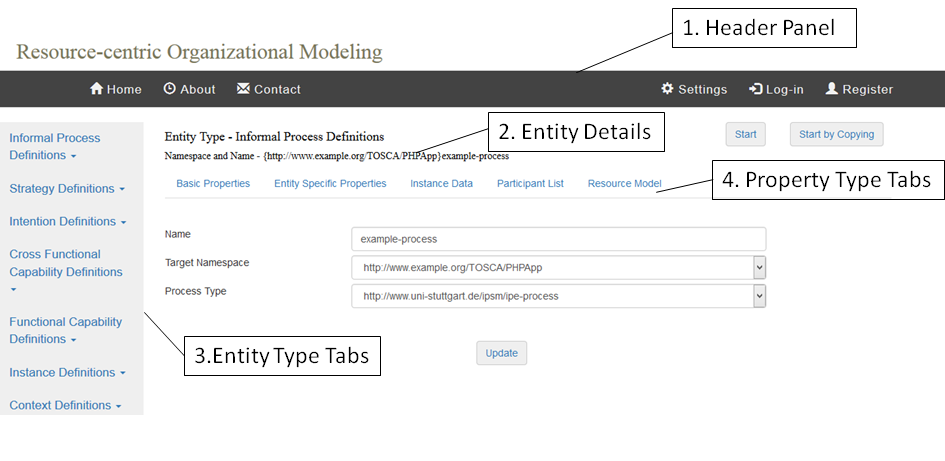
\includegraphics[width=\textwidth,angle=0]{samplescreen.png}
	\caption{Screenshot of Resource Model}
	\label{fig:realizationofresourcemodel}
\end{figure}


\begin{Listing}
	\begin{lstlisting}
	<xs:complexType name="tNodeTemplate">
	<xs:complexContent>
	<xs:extension base="tEntityTemplate">
	<xs:sequence>
	<xs:element name="Requirements" minOccurs="0">
	<xs:complexType>
	<xs:sequence>
	<xs:element name="Requirement" type="tRequirement" maxOccurs="unbounded"/>
	</xs:sequence>
	</xs:complexType>
	</xs:element>
	<xs:element name="Capabilities" minOccurs="0">
	<xs:complexType>
	<xs:sequence>
	<xs:element name="Capability" type="tCapability" maxOccurs="unbounded"/>
	</xs:sequence>
	</xs:complexType>
	</xs:element>
	<xs:element name="Policies" minOccurs="0">
	<xs:complexType>
	<xs:sequence>
	<xs:element name="Policy" type="tPolicy" maxOccurs="unbounded"/>
	</xs:sequence>
	</xs:complexType>
	</xs:element>
	<xs:element name="DeploymentArtifacts" type="tDeploymentArtifacts" minOccurs="0"/>
	</xs:sequence>
	<xs:attribute name="name" type="xs:string" use="optional"/>
	<xs:attribute name="minInstances" type="xs:int" use="optional" default="1"/>
	<xs:attribute name="maxInstances" use="optional" default="1">
	<xs:simpleType>
	<xs:union>
	<xs:simpleType>
	<xs:restriction base="xs:nonNegativeInteger">
	<xs:pattern value="([1-9]+[0-9]*)"/>
	</xs:restriction>
	</xs:simpleType>
	<xs:simpleType>
	<xs:restriction base="xs:string">
	<xs:enumeration value="unbounded"/>
	</xs:restriction>
	</xs:simpleType>
	</xs:union>
	</xs:simpleType>
	</xs:attribute>
	</xs:extension>
	</xs:complexContent>
	</xs:complexType>
	\end{lstlisting}
	\caption{XML Schema Definition of Node Type}
	\label{lst:xsdnodetype}
\end{Listing}
		
%%%%%%%%%%%%%%%%%%%%%%%%%%%%%%%%%%%%%%%%%%%%%%%%%%%%%%%%%%%%%%%%%%%%%%%%%
\subsection{Realization of Instance creation}
%%%%%%%%%%%%%%%%%%%%%%%%%%%%%%%%%%%%%%%%%%%%%%%%%%%%%%%%%%%%%%%%%%%%%%%%%
Initializing resource-centric processes requires acquiring and engaging interrelated resources \cite{Sungur2015}. As mentioned earlier, the phases of compiling and initializing of informal process models are out of scope of this work. Only the functionalities such as creating instances, extracting instances and editing instances are part of the developed editor. This is because initializing informal process models starts after the initial context defined in an IPE model \cite{Sungur2015}. Thus it is important to discuss realization of instance creation which are required for subsequent phases P3 and P4 of Executing Informal Processes (InProXec) method. Acquirable entity types' models can be converted into instances. For example, resource definition is converted into \textit{resource instance}. A model instance contains additional meta-data about the executed processes such as the information about the start date and time, end date and time, instance status, cost, source model etc. From the screen-shot image \ref{fig:realizationofinstances2} it is clear that these properties of an instance can be edited through the developed editor. Only when a acquirable model is successfully initialized it can be engaged to adapt the process execution of emerging requirements \cite{Sungur2015}. The properties that describe each instance is provided in the listing \ref{lst:xsdinstances}

\begin{figure}
	\centering
	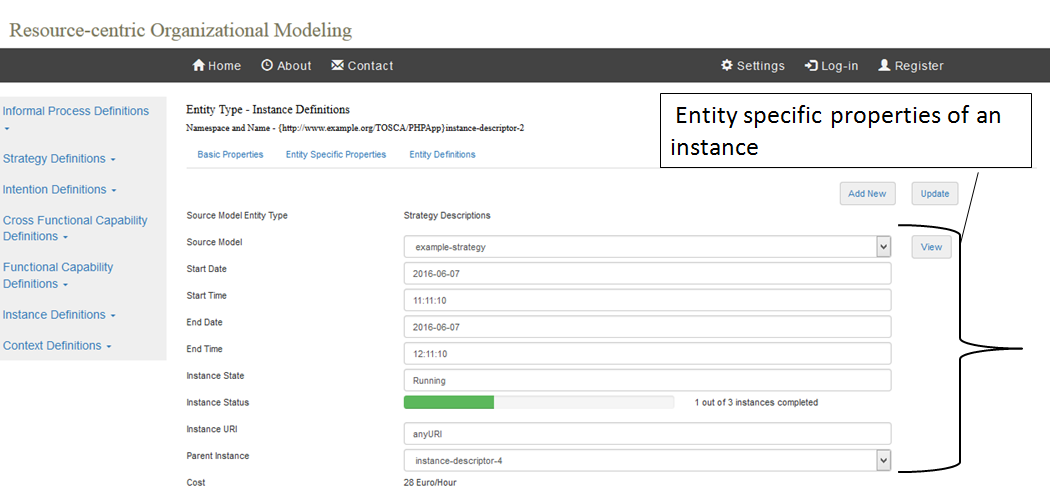
\includegraphics[width=\textwidth,angle=0]{sampleinstancescreen2.png}
	\caption{Screenshot of Instances Descriptor}
	\label{fig:realizationofinstances2}
\end{figure}

The developed editor supports creation and updation of descriptive information about instances. Each instance belong to any one of the acquirable entity type such strategies, intentions and informal processes. Any entity that has instances are also listed inside the \textit{Instance data} tab of each entity. From the screen-shot image Figure \ref{fig:realizationofinstances}, it is clear that the editor has ability to add, remove and extract instance descriptors for any entity type. An instance descriptor of a functional capability refers to a resource definition meaning that a capability is provided by a resource definition. So an instance descriptor of a capability refers to a resource definition.

\begin{figure}
	\centering
	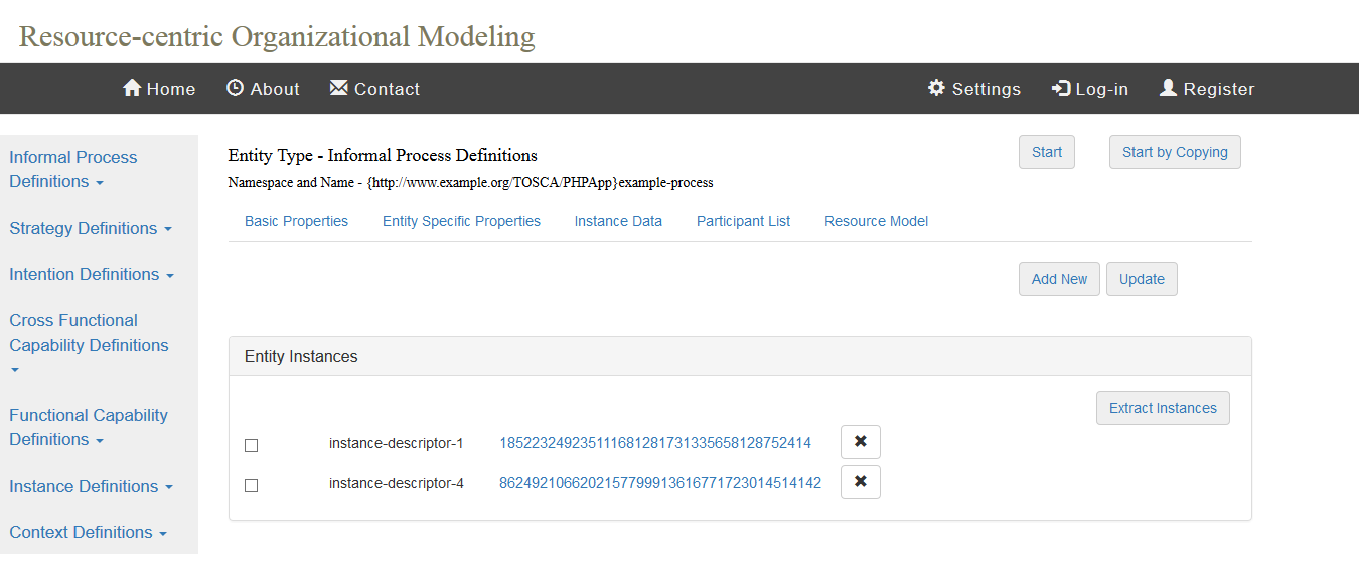
\includegraphics[width=\textwidth,angle=0]{sampleinstancescreen.png}
	\caption{Screenshot of Acquriable Entities}
	\label{fig:realizationofinstances}
\end{figure}


\begin{Listing}
	\begin{lstlisting}
<complexType name="tInstanceDescriptor">
<complexContent>
<extension base="ipsm:tIdentifiableEntityDefinition">
<attribute name="startTime" type="time" use="optional"></attribute>
<attribute name="endTime" type="time" use="optional"></attribute>
<attribute name="instanceState" type="string" use="required"></attribute>
<attribute name="instanceURI" type="anyURI" use="optional"></attribute>
<attribute name="sourceModel" type="tAcquireableentitydefinition" use="required"></attribute>
<attribute name="parentInstance" type="string" use="optional"></attribute>
<attribute name="id" type="string" use="required"></attribute>
<anyAttribute></anyAttribute>
</extension>
</complexContent>
</complexType>		
\end{lstlisting}
\caption{XML Schema Definition of Instance Descriptor}
\label{lst:xsdinstances}
\end{Listing}
		
%%%%%%%%%%%%%%%%%%%%%%%%%%%%%%%%%%%%%%%%%%%%%%%%%%%%%%%%%%%%%%%%%%%%%%%%%
\section{Validation}
\label{sec:validation}
%%%%%%%%%%%%%%%%%%%%%%%%%%%%%%%%%%%%%%%%%%%%%%%%%%%%%%%%%%%%%%%%%%%%%%%%%	
This section validates the degree of satisfaction of the research objectives discussed in Chapter \ref{chap:introduction} by the developed editor. Also, it was claimed in earlier chapters that this master thesis is a part of creating models that are required for supporting and automating informal processes. Hence it is important to evaluate the developed editor along with the requirements that are discussed in the approach \textit{Informal Process Essentials} \cite{Sungur2014a}. In this section, examples are provided from motivating scenario which is discussed in the Chapter \ref{chap:motivatingScenario}. The concept of \textit{resource-centric} modeling approach has also been validated in the approach \textit{Informal Process Essentials} \cite{Sungur2014a}, where the author describes that the approach is right one since the focus is not on business logic rather on other dimensions like resources. The author also states that non-existence of business logic facilitates more autonomy for human performers and enables establishment of best practices. Since the above arguments justifies to the fact of providing more autonomous informal process modeling, one can claim that the approach of \textit{resource-centric modeling} is a valid one. Not stopping with these arguments, a detailed validation of research objectives discussed in Chapter \ref{chap:introduction} and validation of developed editor with suitable examples is provided.
		
%%%%%%%%%%%%%%%%%%%%%%%%%%%%%%%%%%%%%%%%%%%%%%%%%%%%%%%%%%%%%%%%%%%%%%%%%
\subsection{Validation of Research Objectives}
\label{subsec:validationofrequirements}
%%%%%%%%%%%%%%%%%%%%%%%%%%%%%%%%%%%%%%%%%%%%%%%%%%%%%%%%%%%%%%%%%%%%%%%%%
As discussed in Chapter \ref{chap:approach}, the research objectives are satisfied at the design level but their validity can be confirmed only by evaluating the research objectives with some sample scenarios provided in Chapter \ref{chap:motivatingScenario}.   

\textit{Organizational intentions transparency} (R1): A valid user whose credentials are stored in database is able to login successfully and view the intentions and its associated entities. Hence the research objective R1 is met.

\textit{Organizational intention resource-based cost estimation} (R2): An intention whose cost is unspecified for a sample intention, is calculated by the developed system recursively as mentioned in the Chapter \ref{chap:approach}. Thus the research objective R2 is also met.

\textit{Organizational intention achievability estimation} (R3): Similar to cost calculation, an intention instance whose achieve-ability not known in prior is also estimated by the current functioning system. Hence research objective R3 is satisfied.

\textit{Intention oriented working style} (R4): The users can login and create intention models, strategy models, informal process models etc., through the developed editor. Hence research objective R4 is also met.

\textit{Participative organizational modeling} (R5): Each entity type that can be interactively acquirable has list of participants with their corresponding privileges. Thus this satisfies the requirements of research objective R5.

\textit{Re-use of organizational knowledge} (R6): The descriptive information about each models can be stored and re-used for next enactments. Hence research objective R6 is also met.
	
